In this Section, the multiclass kernel perceptron algorithm presented in the theory part above is trained on the training set $S$ of the MNIST dataset for several settings. The multiclass predictors are trained using the three different realizations of the multiclass kernel perceptron algorithm. The performance of the trained multiclass predictors is evaluated on the test set $D$. The test error rates of the three realizations of the multiclass kernel perceptron algortihm are compared for different choices of the degree of the polynomial kernel $p$. In the present work, degrees from $p=1$ up to $p=6$ are applied. Each predictor is trained for a total of $N_{epoch}=10$ cycles over random permutations of the training examples in the training set $S$. The final result are three multiclass predictors - one for each realization of the multiclass kernel perceptron algorithm - that minimize the test error rate on the test set $D$.

\subsection{Binary Predictors}\label{subsec:bin_pred}
Before presenting the obtained multiclass predictors, it is instructive to take a look at what happens at the heart of the multiclass kernel perceptron algorithm when performing a training on the training set $S$. As explained in the theory part, the multiclass kernel perceptron algorithm is a simple combination of ten binary predictors - one for each digit $a$. Here, exemplarily, the binary predictor $h_{S^{(5)}}$ for the digit $a=5$ is considered. Nonetheless, the key statements in this Subsection are valid for all of the ten digits. \\

Figure~\ref{fig:train_error_bin} shows the binary training error rates $\hat{\ell}_{S^{(5)}}$ as a function of the number of epochs $N_{epoch}$ for the six different degrees $p$ of the polynomial kernel. In each panel, the binary training error rates $\hat{\ell}_{S^{(5)}}$ for the final $\vec{\alpha}_{fin}$, the minimizing $\vec{\alpha}_{min}$, and the average predictor $\langle\vec{\alpha}\rangle$ are displayed. The test error rates $\hat{\ell}_{D^{(5)}}$ for the same binary predictors are reported in Fig.~\ref{fig:test_error_bin}. \\

For the binary predictors with a linear kernel ($p=1$), the binary training error rate $\hat{\ell}_{S^{(5)}}$ remains constant roughly between \SI{2}{\percent} and \SI{4}{\percent} with respect to the number of epochs $N_{epoch}$. Especially, the binary kernel perceptron algorithm does not terminate, i.e. it does not reach a training error rate of \SI{0}{\percent}. It is well-known that the binary perceptron algorithm presented by Rosenblatt is only guaranteed to terminate on linearly separable training sets. Given the complexity of the MNIST dataset and the obtained training error rates $\hat{\ell}_{S^{(5)}}$, it is concluded that the binary training set $S^{(5)}$ is not linearly separable. For higher degrees $p$, a convergence of the training error rate $\hat{\ell}_{S^{(5)}}$ to lower values, and even to \SI{0}{\percent} is observed. This is especially true for kernels with a degree of $p=3$ or more. The number of epochs $N_{epoch}$ required for the convergence of the training error rate $\hat{\ell}_{S^{(5)}}$ decreases with the degree $p$ of the polynomial kernel.

\begin{figure}[hbt!]
    \begin{subfigure}[t]{0.49\textwidth}
        \centering
        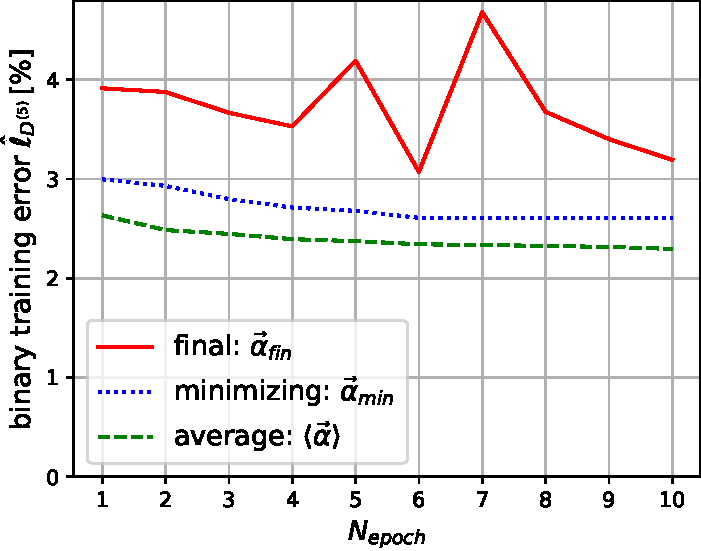
\includegraphics[width=\linewidth]{bin_pred/training_digit=5_deg=1.pdf} 
        \caption{$p = 1$}
    \end{subfigure}
    \hfill
    \begin{subfigure}[t]{0.49\textwidth}
        \centering
        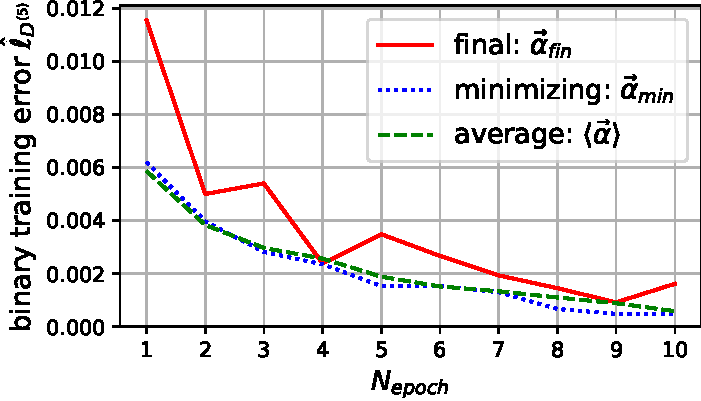
\includegraphics[width=\linewidth]{bin_pred/training_digit=5_deg=2.pdf} 
        \caption{$p = 2$}
    \end{subfigure}
    \par\bigskip
        \begin{subfigure}[t]{0.49\textwidth}
        \centering
        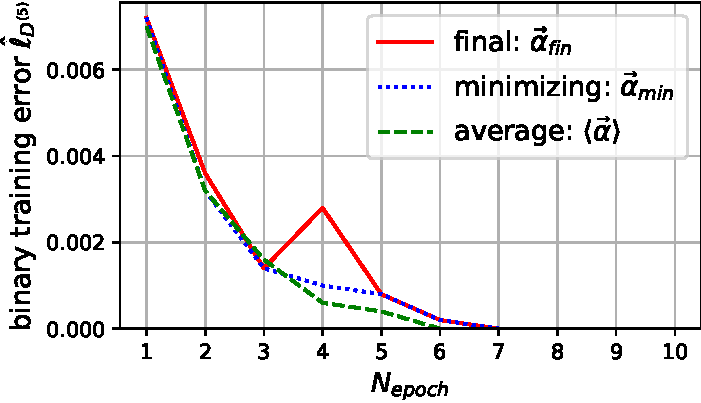
\includegraphics[width=\linewidth]{bin_pred/training_digit=5_deg=3.pdf} 
        \caption{$p = 3$}
    \end{subfigure}
    \hfill
    \begin{subfigure}[t]{0.49\textwidth}
        \centering
        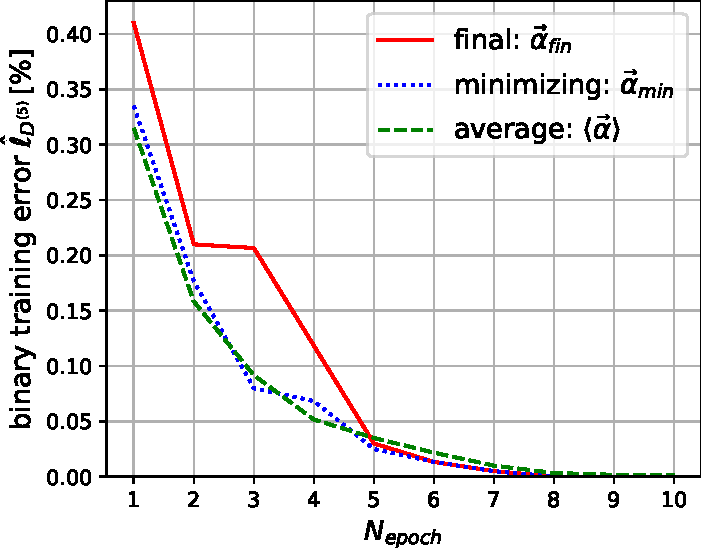
\includegraphics[width=\linewidth]{bin_pred/training_digit=5_deg=4.pdf} 
        \caption{$p = 4$}
    \end{subfigure}
    \par\bigskip
        \begin{subfigure}[t]{0.49\textwidth}
        \centering
        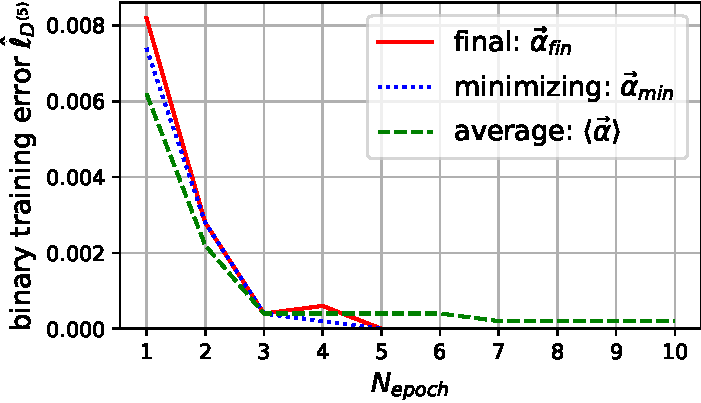
\includegraphics[width=\linewidth]{bin_pred/training_digit=5_deg=5.pdf} 
        \caption{$p = 5$}
    \end{subfigure}
    \hfill
    \begin{subfigure}[t]{0.49\textwidth}
        \centering
        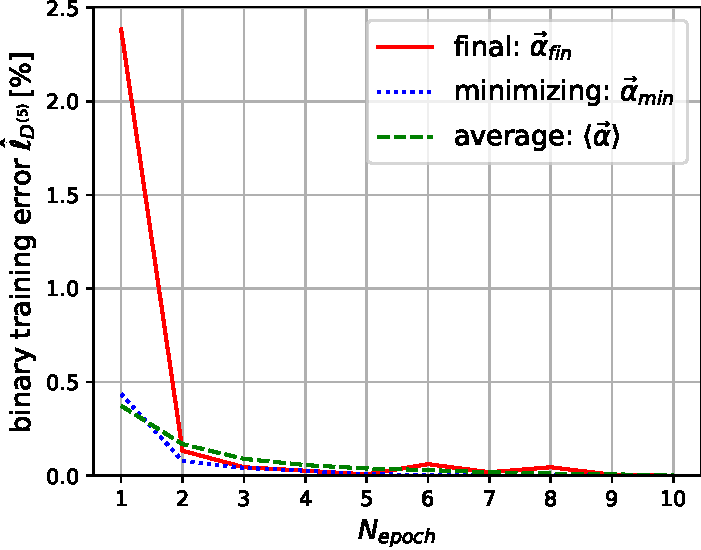
\includegraphics[width=\linewidth]{bin_pred/training_digit=5_deg=6.pdf} 
        \caption{$p = 6$}
    \end{subfigure}
    \caption{Binary training error rates $\hat{\ell}_{S^{(5)}}$ as a function of the number of epochs $N_{epoch}$ for the training of binary predictors that classify, whether an image shows the digit $a=5$ or not. Each panel displays the binary training error rates $\hat{\ell}_{S^{(5)}}$ for a different degree $p$ of the polynomial kernel for the three approaches to retrieve binary predictors from the binary kernel perceptron algorithm. Note, the different scales of the vertical axes. The binary test error $\hat{\ell}_{D^{(5)}}$ rates for the same binary predictors are displayed in Fig~\ref{fig:test_error_bin}.}\label{fig:train_error_bin}
\end{figure}

\begin{figure}[h!]
    \begin{subfigure}[t]{0.49\textwidth}
        \centering
        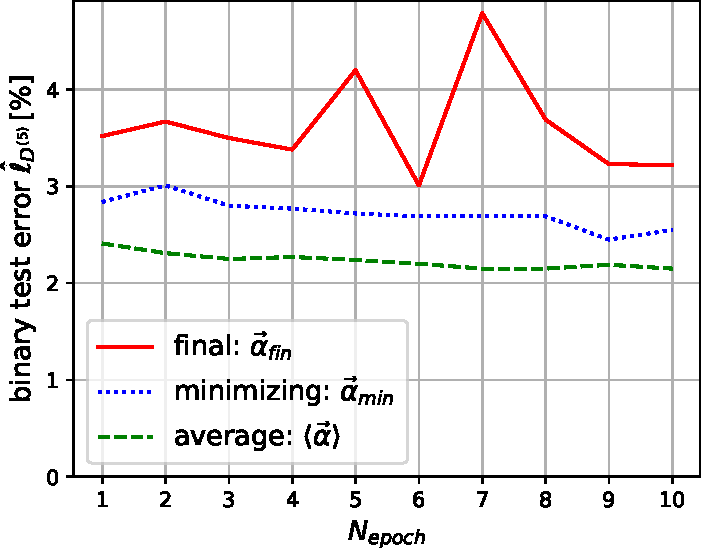
\includegraphics[width=\linewidth]{bin_pred/test_digit=5_deg=1.pdf} 
        \caption{$p = 1$}
    \end{subfigure}
    \hfill
    \begin{subfigure}[t]{0.49\textwidth}
        \centering
        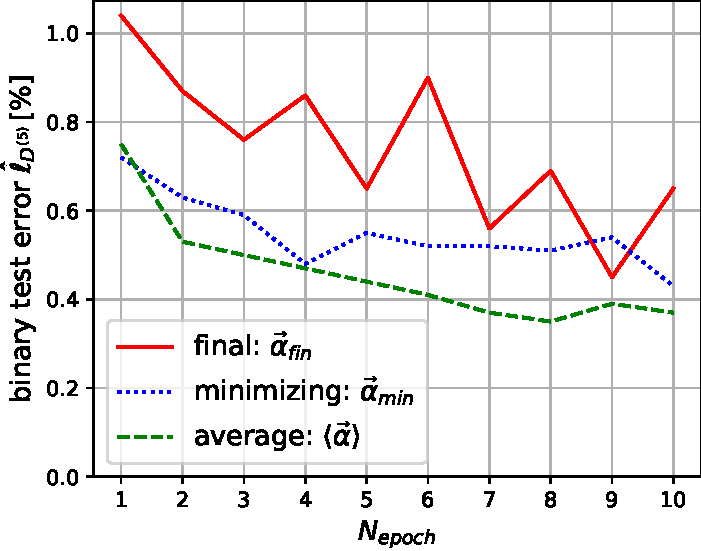
\includegraphics[width=\linewidth]{bin_pred/test_digit=5_deg=2.pdf} 
        \caption{$p = 2$}
    \end{subfigure}
    \par\bigskip
        \begin{subfigure}[t]{0.49\textwidth}
        \centering
        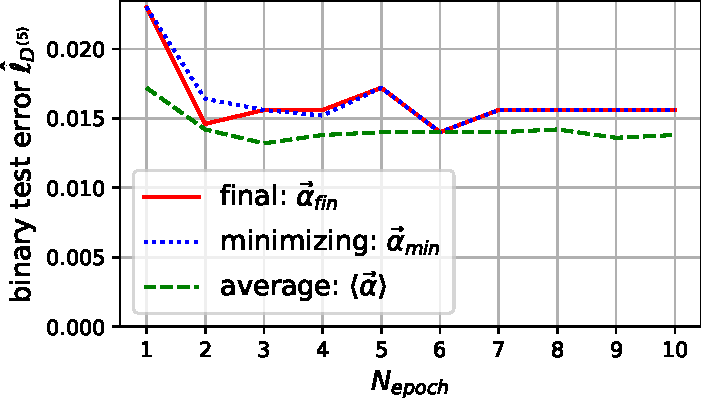
\includegraphics[width=\linewidth]{bin_pred/test_digit=5_deg=3.pdf} 
        \caption{$p = 3$}
    \end{subfigure}
    \hfill
    \begin{subfigure}[t]{0.49\textwidth}
        \centering
        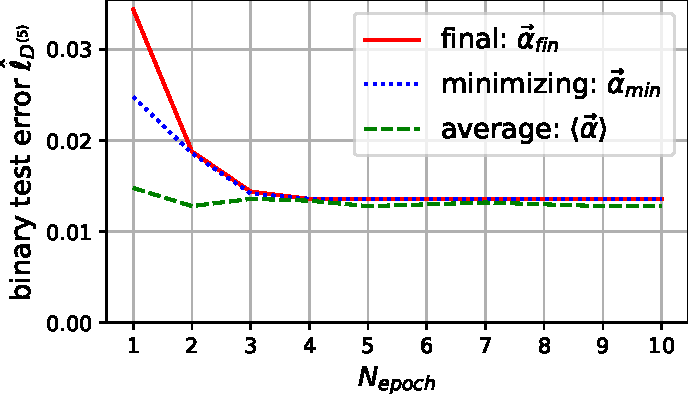
\includegraphics[width=\linewidth]{bin_pred/test_digit=5_deg=4.pdf} 
        \caption{$p = 4$}
    \end{subfigure}
    \par\bigskip
        \begin{subfigure}[t]{0.49\textwidth}
        \centering
        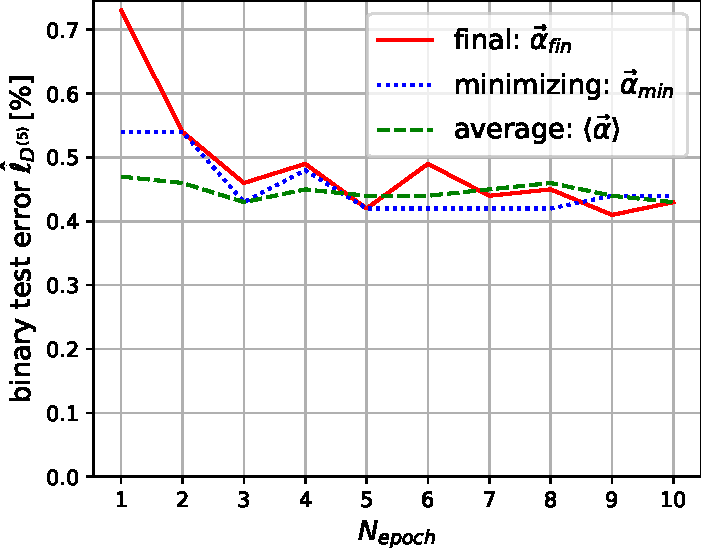
\includegraphics[width=\linewidth]{bin_pred/test_digit=5_deg=5.pdf} 
        \caption{$p = 5$}
    \end{subfigure}
    \hfill
    \begin{subfigure}[t]{0.49\textwidth}
        \centering
        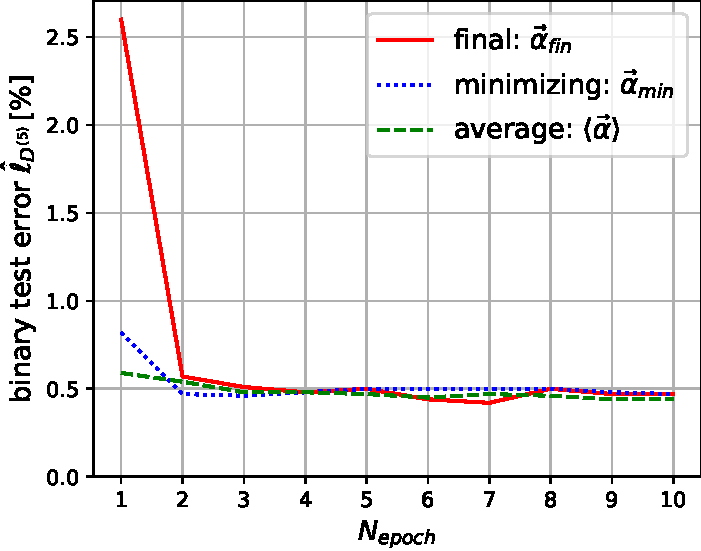
\includegraphics[width=\linewidth]{bin_pred/test_digit=5_deg=6.pdf} 
        \caption{$p = 6$}
    \end{subfigure}
    \caption{Binary test error rates $\hat{\ell}_{D^{(5)}}$ as a function of the number of epochs $N_{epoch}$ for the training of binary predictors that classify, whether an image shows the digit $a=5$ or not. Each panel displays the binary test error rates $\hat{\ell}_{D^{(5)}}$ for a different degree $p$ of the polynomial kernel for the three approaches to retrieve binary predictors from the binary kernel perceptron algorithm. Note, the different scales of the vertical axes. The binary training error rates $\hat{\ell}_{S^{(5)}}$ for the same binary predictors are displayed in Fig~\ref{fig:train_error_bin}.} \label{fig:test_error_bin}
\end{figure}

Regarding the three different binary predictor types $\vec{\alpha}_{fin}$, $\vec{\alpha}_{min}$, and $\langle\vec{\alpha}\rangle$, the final predictor $\vec{\alpha}_{fin}$ reveals the less smooth curve. This observation is caused by the fact that the final predictor $\vec{\alpha}_{fin}$ is highly biased by the latest training examples in each epoch. Typically, the minimizing and the average predictors, $\vec{\alpha}_{min}$ and $\langle\vec{\alpha}\rangle$, have a lower training error rate $\hat{\ell}_{S^{(5)}}$ than the final predictor $\vec{\alpha}_{fin}$, given a certain number of epochs $N_{epoch}$ and a degree $p$ of the polynomial kernel. \\

Interestingly, the training error rate $\hat{\ell}_{S^{(5)}}$ for the average predictor $\langle\vec{\alpha}\rangle$ can be lower than the training error rate $\hat{\ell}_{S^{(5)}}$ of the minimizing predictor $\vec{\alpha}_{min}$. The reason for this observation is that the minimizing predictor $\vec{\alpha}_{min}$ searches for the predictor that minimizes the training error rate $\hat{\ell}_{S^{(5)}}$ among the predictors $\vec{\alpha}$ that are produced during the training phase of the binary kernel perceptron algorithm, compare Alg.~\ref{alg:binary_kernel_perceptron}. The average predictor $\langle\vec{\alpha}\rangle$ is not included in this set, and can thus have a lower training error rate $\hat{\ell}_{S^{(5)}}$. However, the training error rate $\hat{\ell}_{S^{(5)}}$ of the minimizing predictor $\vec{\alpha}_{min}$ is always lower than the one of the final predictor $\vec{\alpha}_{fin}$. In general, the dependence of the training error rate $\hat{\ell}_{S^{(5)}}$ for the minimizing and the average predictor, $\vec{\alpha}_{min}$ and $\langle\vec{\alpha}\rangle$, are comparable, though the average predictor leads to a slightly smoother curve.\\

A closer look at the corresponding binary test error rates in Fig.~\ref{fig:test_error_bin} reveals that the test error rate $\hat{\ell}_{D^{(5)}}$ saturates at values significantly larger than \SI{0}{\percent} for all degrees $p$ of the polynomial kernel. For the lowest four degrees $p$ of the polynomial kernel, a notably decrease of the binary test error rates $\hat{\ell}_{D^{(5)}}$ is observed. For the degrees $p\geq 5$, the test error rate for all the three predictor types does not drop below roughly \SI{0.5}{\percent}. Here, the polynomial kernel overfits, such that an excellent performance on the training set $S^{(5)}$, but a rather poor performance on the test set $D^{(5)}$ is obtained. In general, the saturation of the test error rate $\hat{\ell}_{D^{(5)}}$ as a function of $N_{epoch}$ implies that the application of the binary kernel perceptron algorithm using a polynomial kernel does not lead to arbitrary accurate binary predictors, as suggested by the training error rate $\hat{\ell}_{S^{(5)}}$.

\subsection{Multiclass Predictors}\label{subsec:multi_pred}
In order to obtain multiclass predictors from the multiclass kernel perceptron algorithm, the ten binary predictors for each digit $a$ are combined. Fig.~\ref{fig:train_error_multi} reports the multiclass training error rates $\hat{\ell}_S$ as a function of the number of epochs $N_{epoch}$ for the three different predictor types. Each panel corresponds to a different degree $p$ of the polynomial kernel that is applied to train the multiclass kernel perceptron algorithm. The test error rate $\hat{\ell}_D$ of the same multiclass predictors can be found in Fig.~\ref{fig:test_error_multi}.\\

Unsurprisingly, the results for the multiclass predictors here reveal similar features as the binary training and test error rates for the binary predictors, reported in the last subsection. The polynomial kernel with less than $p = 3$ degrees leads to slow convergence of the multiclass training error rate $\hat{\ell}_S$ as a function of $N_{epoch}$ as well as to comparably high test error rates $\hat{\ell}_D$. Especially for $p=1$, the multiclass predictor underfits the data clearly, as both the training and test error rates are comparably large, and do not decrease with the number of epochs $N_{epoch}$. Polynomial kernels with a degree of at least $p=3$ do not improve the test error rate, but also do not reduce the performance notably, i.e., for the applied degrees $p$, the polynomial kernel does not overfit the data strongly. In contrast to the binary predictors, here, the training error rate $\hat{\ell}_S$ of the minimizing predictor $\vec{\alpha}_{min}$ is lower than the one of the average predictor $\langle\vec{\alpha}\rangle$. For the test error rate $\hat{\ell}_D$, the final predictor $\vec{\alpha}_{min}$ performance typically worse than the other two realizations of the multiclass kernel perceptron algorithm.

\begin{figure}[h!]
    \begin{subfigure}[t]{0.49\textwidth}
        \centering
        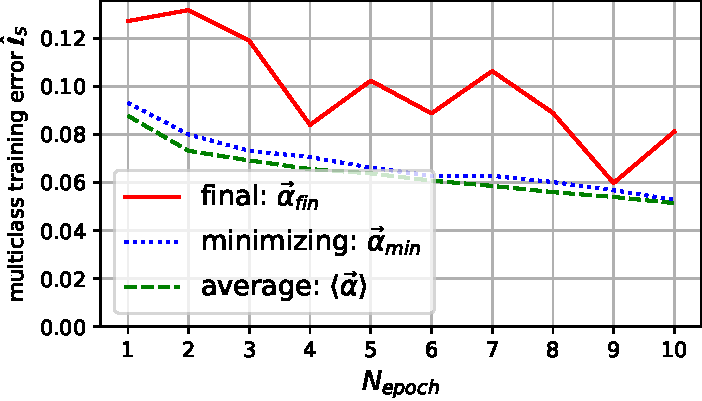
\includegraphics[width=\linewidth]{performance/training_deg=1.pdf} 
        \caption{$p = 1$}
    \end{subfigure}
    \hfill
    \begin{subfigure}[t]{0.49\textwidth}
        \centering
        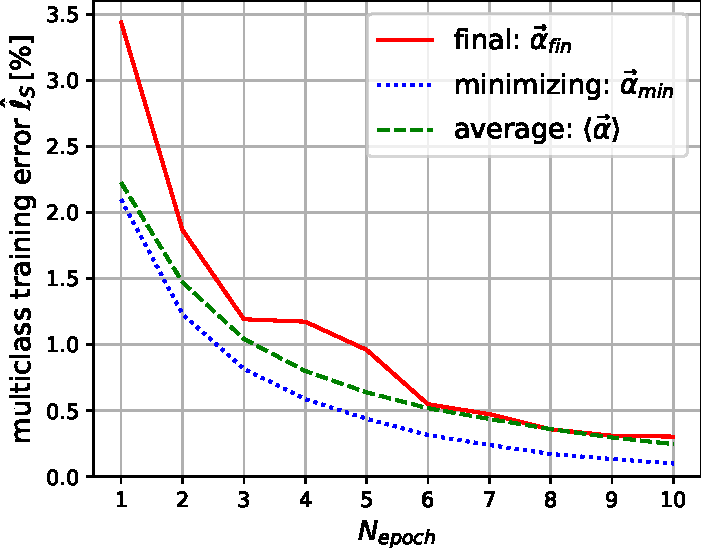
\includegraphics[width=\linewidth]{performance/training_deg=2.pdf} 
        \caption{$p = 2$}
    \end{subfigure}
    \par\bigskip
        \begin{subfigure}[t]{0.49\textwidth}
        \centering
        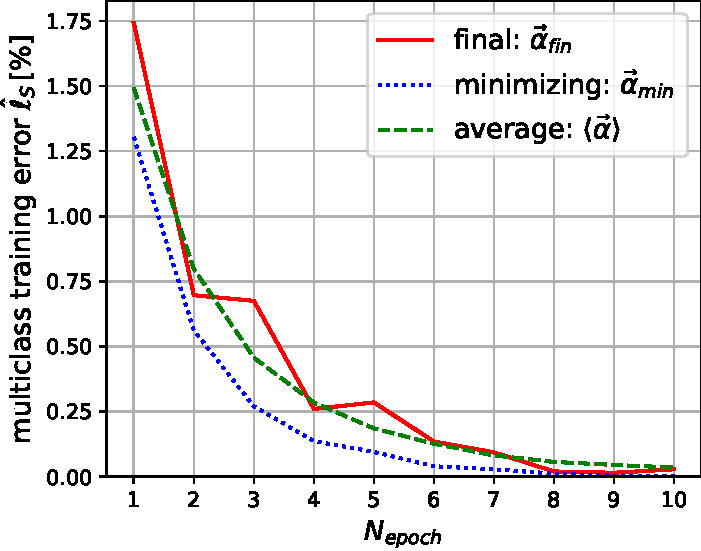
\includegraphics[width=\linewidth]{performance/training_deg=3.pdf} 
        \caption{$p = 3$}
    \end{subfigure}
    \hfill
    \begin{subfigure}[t]{0.49\textwidth}
        \centering
        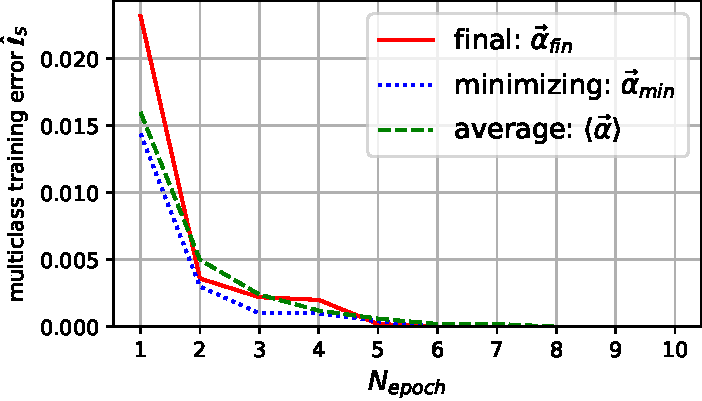
\includegraphics[width=\linewidth]{performance/training_deg=4.pdf} 
        \caption{$p = 4$}
    \end{subfigure}
    \par\bigskip
        \begin{subfigure}[t]{0.49\textwidth}
        \centering
        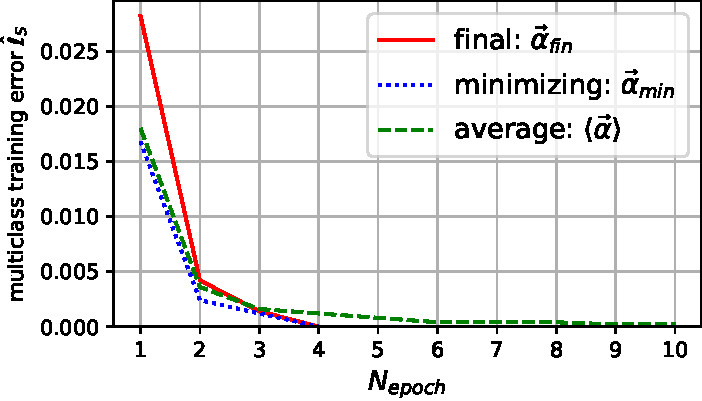
\includegraphics[width=\linewidth]{performance/training_deg=5.pdf} 
        \caption{$p = 5$}
    \end{subfigure}
    \hfill
    \begin{subfigure}[t]{0.49\textwidth}
        \centering
        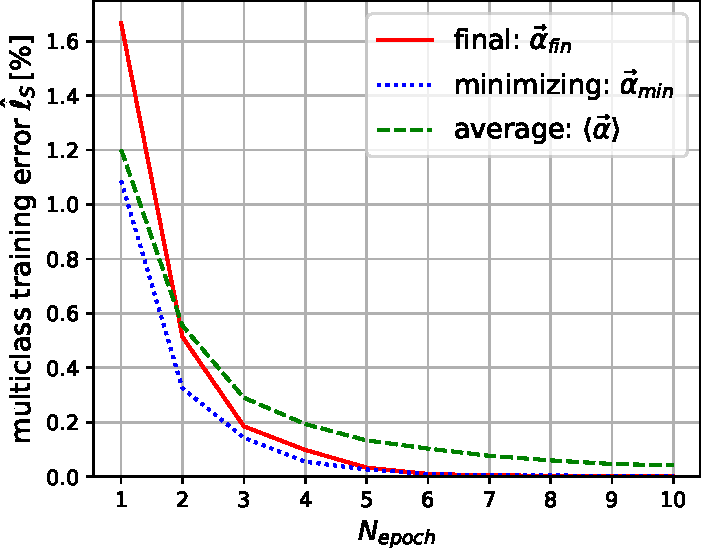
\includegraphics[width=\linewidth]{performance/training_deg=6.pdf} 
        \caption{$p = 6$}
    \end{subfigure}
    \caption{Multiclass training error rates $\hat{\ell}_{S}$ as a function of the number of epochs $N_{epoch}$ for the training of multiclass predictors on the MNIST training set $S$. The multiclass predictors classify given images of handwritten digits with a label between $0$ and $9$. Each panel displays the multiclass training error rates $\hat{\ell}_{S}$ for a different degree $p$ of the polynomial kernel for the three approaches to retrieve binary predictors inside the multiclass kernel perceptron algorithm. Note, the different scales of the vertical axes. The multiclass test error rates $\hat{\ell}_{D}$ for the same multiclass predictors are displayed in Fig~\ref{fig:test_error_multi}.}
    \label{fig:train_error_multi}
\end{figure}

\begin{figure}[h!]
    \begin{subfigure}[t]{0.49\textwidth}
        \centering
        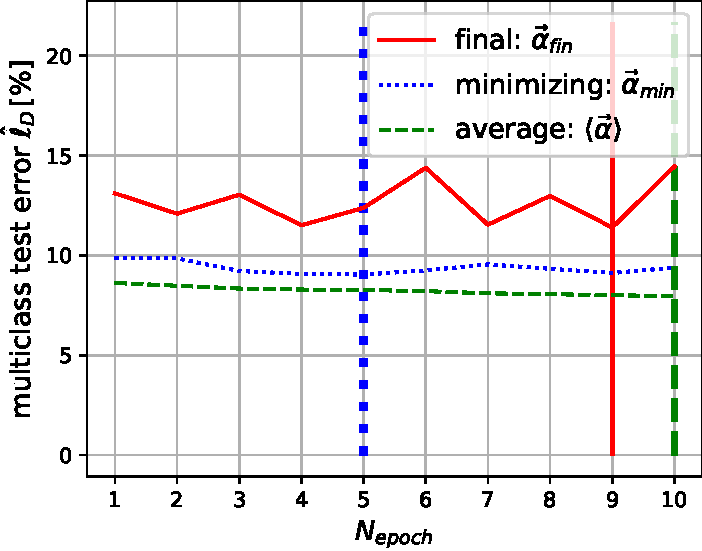
\includegraphics[width=\linewidth]{performance/test_deg=1.pdf} 
        \caption{$p = 1$}
    \end{subfigure}
    \hfill
    \begin{subfigure}[t]{0.49\textwidth}
        \centering
        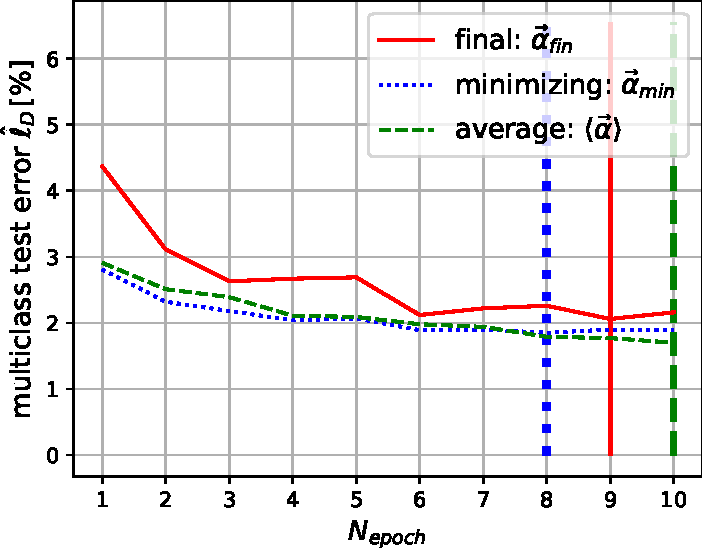
\includegraphics[width=\linewidth]{performance/test_deg=2.pdf} 
        \caption{$p = 2$}
    \end{subfigure}
    \par\bigskip
        \begin{subfigure}[t]{0.49\textwidth}
        \centering
        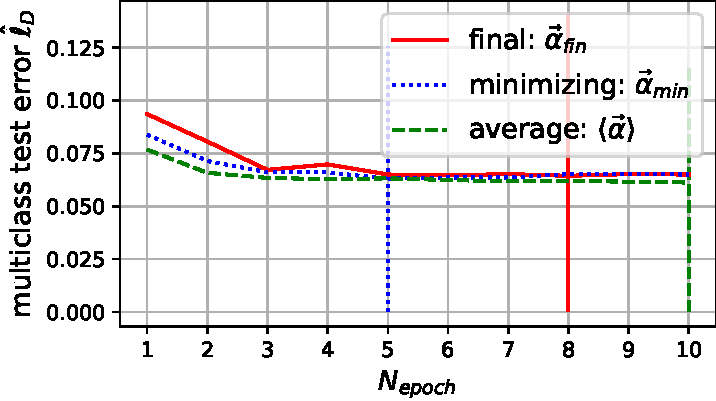
\includegraphics[width=\linewidth]{performance/test_deg=3.pdf} 
        \caption{$p = 3$}
    \end{subfigure}
    \hfill
    \begin{subfigure}[t]{0.49\textwidth}
        \centering
        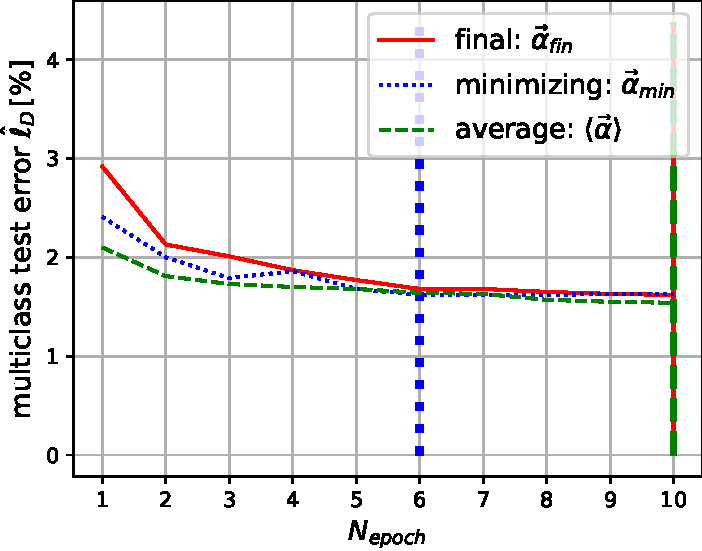
\includegraphics[width=\linewidth]{performance/test_deg=4.pdf} 
        \caption{$p = 4$}
    \end{subfigure}
    \par\bigskip
        \begin{subfigure}[t]{0.49\textwidth}
        \centering
        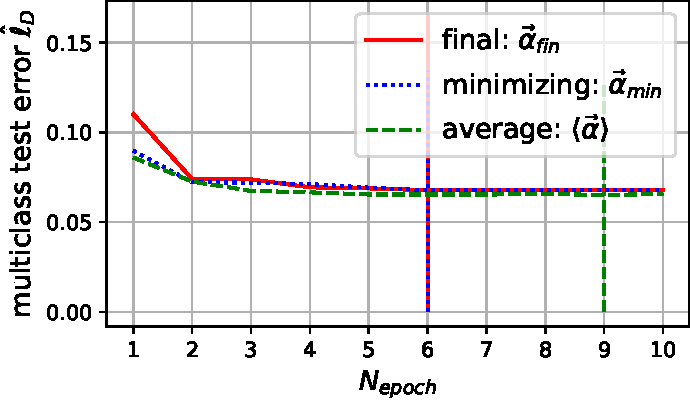
\includegraphics[width=\linewidth]{performance/test_deg=5.pdf} 
        \caption{$p = 5$}
    \end{subfigure}
    \hfill
    \begin{subfigure}[t]{0.49\textwidth}
        \centering
        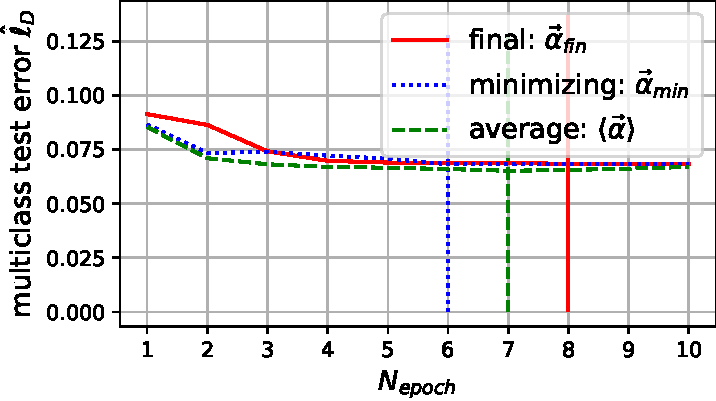
\includegraphics[width=\linewidth]{performance/test_deg=6.pdf} 
        \caption{$p = 6$}
    \end{subfigure}
    \caption{Multiclass test error rates $\hat{\ell}_{D}$ as a function of the number of epochs $N_{epoch}$ for the training of multiclass predictors on the MNIST training set $S$. The multiclass predictors classify given images of handwritten digits with a label between $0$ and $9$. Each panel displays the multiclass test error rates $\hat{\ell}_{D}$ for a different degree $p$ of the polynomial kernel for the three approaches to retrieve binary predictors inside the multiclass kernel perceptron algorithm. Note, the different scales of the vertical axes. The multiclass training error rates $\hat{\ell}_{S}$ for the same multiclass predictors are displayed in Fig~\ref{fig:train_error_multi}. In each panel, the vertical lines indicate the number of epochs $N_{epoch}$ with the smallest test error rate for all three predictor types. The predictors obtaining overall the lowest test error rates are reported in Tab.~\ref{tab:min_test}.}
    \label{fig:test_error_multi}
\end{figure}

\clearpage

\subsection{Minimizing the Test Error Rate}\label{subsec:best_pred}
In the previous subsection, the multiclass test error rates $\hat{\ell}_D$ of several multiclass predictors trained on $S$ using the multiclass kernel perceptron algorithm were presented. In Tab.~\ref{tab:min_test}, for each of the three predictor types, the degree $p$ of the polynomial kernel as well as the absolved number of epochs $N_{epoch}$ for which the test error rate $\hat{\ell}_D$ is minimized is reported. For completeness, also the obtained training error rate $\hat{\ell}_S$ is stated. These three classifiers reveal the highest performance for the identification of handwritten digits in the MNIST dataset, and are the final result of the present work. As already observed, the final predictor $\vec{\alpha}_{fin}$ has a larger test error rate $\hat{\ell}_D$ than the minimizing and average predictor, $\vec{\alpha}_{min}$ and $\langle\vec{\alpha}\rangle$.

\begin{table}[h!]
\centering
\begin{tabular}{c||c|c|c}
& $\vec{\alpha}_{fin}$ & $\vec{\alpha}_{min}$ & $\langle \vec{\alpha} \rangle$\\
\hline
\hline
$\hat{\ell}_D\,[\%]$ & \boldmath$1.58$ & \boldmath$1.55$ & \boldmath$1.54$\\
$\hat{\ell}_S\,[\%]$ & $0.0150$ & $0.127$ & $0.0200$ \\
$p$ & $3$ & $3$ & $4$\\
$N_{epoch}$ & $9$ & $6$ & $10$
\end{tabular}
\caption{Multiclass predictors that obtain the lowest test error rates $\hat{\ell}_D$ on the test set $D$ of the MNIST database of handwritten digits applying the multiclass kernel perceptron algorithm. In the table, the degree $p$ of the polynomial kernel as well as the number of epochs $N_{epoch}$ for which the test error rate $\hat{\ell}_D$ is minimized are stated for each of the three predictor types $\vec{\alpha}_{fin}$, $\vec{\alpha}_{min}$, and $\langle\vec{\alpha}\rangle$. In the present work, kernel degrees from $p=1$ to $p=6$ for up to $N_{epoch}=10$ training cycles over random permuations in the training set $S$ were considered. For completeness, the corresponding training error rate $\hat{\ell}_S$ is reported.}
\label{tab:min_test}
\end{table}

Finally, in Fig.~\ref{fig:conf_mat}, the confusion matrix for the three multiclass predictors with the lowest test error rates $\hat{\ell}_D$ are reported. Clearly, all the predictors perform well on the test set $D$. There is no particular digit for which a particular large number of missclassifications is observed. This refers to the observation in Sec.~\ref{sec:dataset_definitions} that the training set $S$ is balanced. Therefore, there is no bias towards particular digits, and for all ten digits roughly the same amount of information is available. 

\begin{figure}
\centering
	\begin{subfigure}[t]{0.49\textwidth}
	\centering
		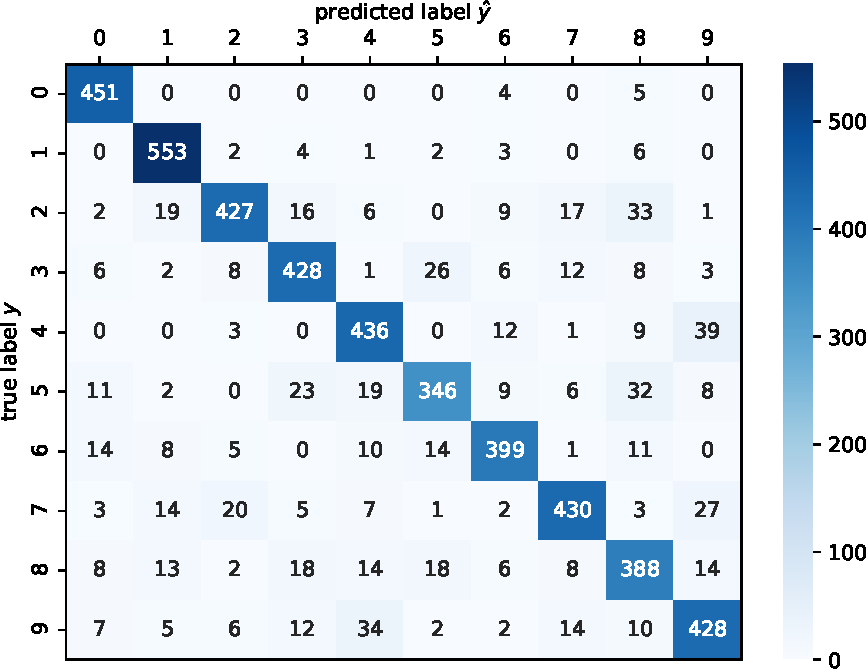
\includegraphics[width=\linewidth]{conf_mat/predictor.pdf} 
		\caption{final predictor $\vec{\alpha}_{fin}$}
	\end{subfigure}
	\hfill
	\begin{subfigure}[t]{0.49\textwidth}
	\centering
		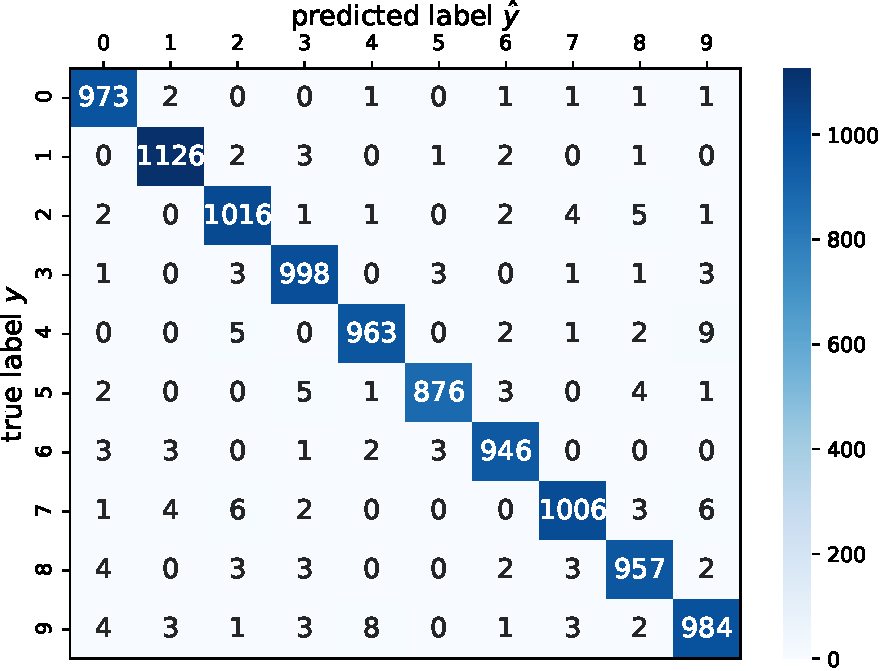
\includegraphics[width=\linewidth]{conf_mat/min_predictor.pdf} 
		\caption{minimizing predictor $\vec{\alpha}_{min}$}
	\end{subfigure}
		\begin{subfigure}[t]{0.49\textwidth}
	\centering
		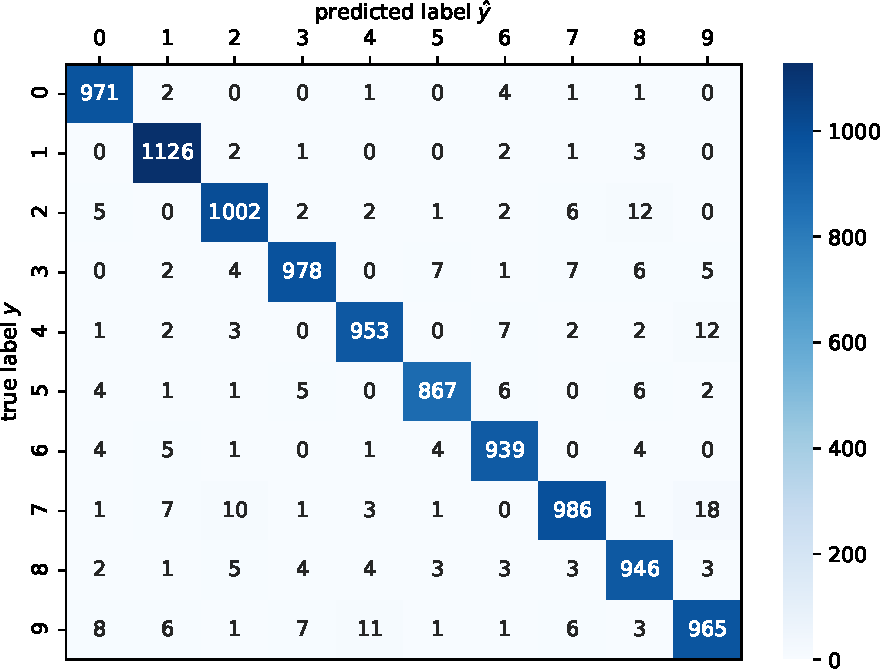
\includegraphics[width=\linewidth]{conf_mat/avg_predictor.pdf} 
		\caption{average predictor $\langle\vec{\alpha}\rangle$}
	\end{subfigure}
	\caption{Confusion matrix for the multiclass predictor that minimizes the test error rate $\hat{\ell}_D$ on the test set $D$ of the MNIST database, for (a) the final predictor $\vec{\alpha}_{fin}$, (b) the minimizing predictor $\vec{\alpha}_{min}$, and (c) the average predictor $\langle\vec{\alpha}\rangle$, as reported in Tab.~\ref{tab:min_test}.}\label{fig:conf_mat}
\end{figure}